\documentclass[spanish]{beamer}

%%% CODIFICACIÓN

\usepackage[utf8]{inputenc}
\usepackage[spanish]{babel}
\usepackage{graphics,tikz}
\graphicspath{{./fig/}}
%%% FUENTES

\usepackage[T1]{fontenc}
\usepackage[familydefault,regular]{}
\usepackage{newtxsf} % Fuente de matemáticas

\setbeamertemplate{navigation symbols}{}

%%% COLORES

\definecolor{background}{RGB}{255,255,255}
\definecolor{text}{RGB}{78,78,78}
\definecolor{accent}{RGB}{6, 105, 125}

\setbeamerfont{framesubtitle}{size=\normalfont\tiny}
\setbeamercolor{framesubtitle}{fg=white}


%%% AJUSTES DE BEAMER

% ¿Negrita en el título de diapositiva o no?
%\setbeamertemplate{frametitle}{\color{accent}\vspace*{1cm}\bfseries\insertframetitle\par\vskip-6pt}

\setbeamertemplate{frametitle}{\color{accent}\vspace*{1cm}\insertframetitle\par\vskip-6pt}

\setbeamertemplate{itemize items}[circle] % Viñetas de itemize

%%% CONFIGURACIÓN DE COLORES DE BEAMER

\setbeamercolor{background canvas}{bg=background}
\setbeamercolor{normal text}{fg=text}
\setbeamercolor{alerted text}{fg=accent}
\setbeamercolor{block title}{fg=accent}
\setbeamercolor{alerted text}{fg=accent}
\setbeamercolor{itemize item}{fg=accent}
\setbeamercolor{enumerate item}{fg=accent}
\setbeamercolor*{title}{fg=accent}
\setbeamercolor{caption name}{fg=accent}
\setbeamercolor{qed symbol}{fg=accent}
\setbeamercolor{itemize subitem}{fg=accent}
\setbeamercolor{bibliography entry author}{fg=text}
\setbeamertemplate{itemize subitem}[triangle]
\usebeamercolor[fg]{normal text}

%%% INFORMACIÓN DEL DOCUMENTO

\title{\textit{Clustering}}
\subtitle{Estadística Multivariante}
\author{Sofía Almeida Bruno\\ Daniel Bolaños Martínez\\ José María Borrás Serrano\\ Fernando de la Hoz Moreno\\ Pedro Manuel Flores Crespo\\ María Victoria Granados Pozo}


\begin{document}

\maketitle
	
\begin{frame}{\textit{Clustering}}
  \begin{itemize}
  \item Objetivo: agrupar objetos similares.
  \item Dadas \textbf{$x_1$}$,\cdots, $\textbf{$x_n$} medidas de $p$ variables en $n$ objetos considerados \textit{heterogéneos}. El objetivo del análisis clúster es agrupar estos objetos en $k$ clases \textit{homogéneas}, donde $k$ es también desconocido.
  \end{itemize}
\end{frame}

\begin{frame}{\textit{Clustering}}
\begin{figure}[H]
	\centering
	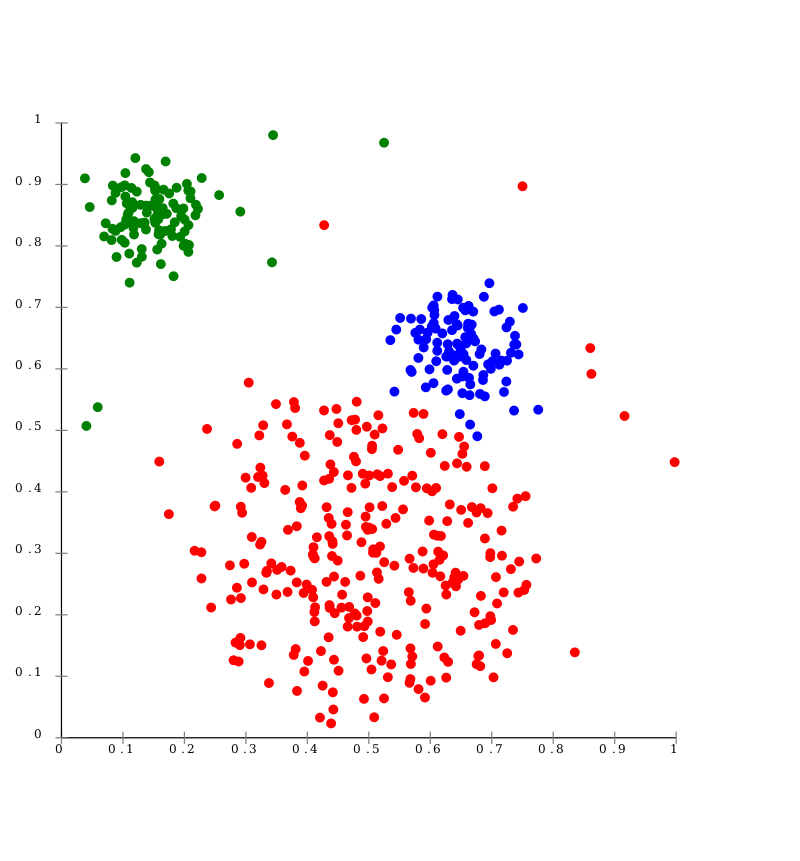
\includegraphics[scale=0.2]{ejemplo}
	\caption{Ejemplo de \textit{clustering}. \cite{chire_deutsch:_2011}}
	\label{fig:ejemplo1}
\end{figure}
\end{frame}

\begin{frame}{Ejemplos de \textit{Clustering}}
  \begin{itemize}
  \item Biología: determinación de especies.
  \item \textit{Marketing}: descubrimiento de grupos de clientes.
    \begin{figure}[H]
	\centering
	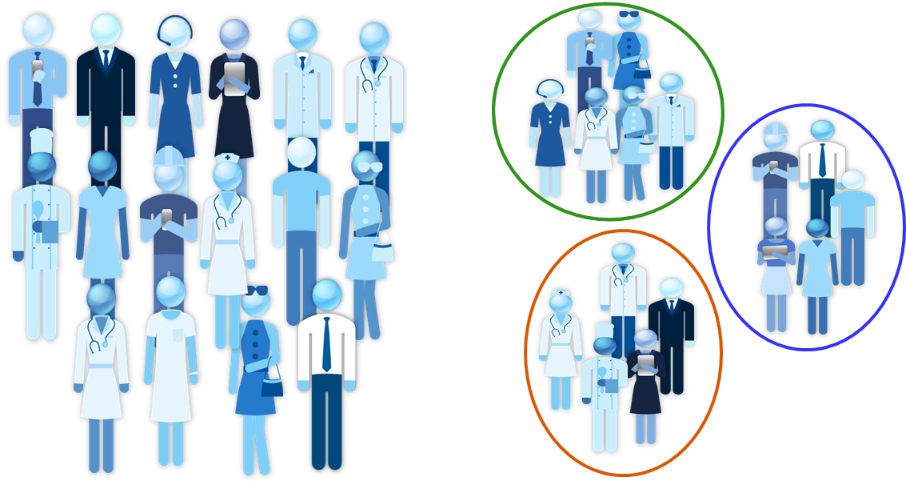
\includegraphics[scale=0.5]{ej_marketing}
	\caption{Ejemplo de \textit{clustering}. \cite{noauthor_understanding_nodate}}
\end{figure}
  \item Psicología: encontrar tipos de personalidad.
  \item Arqueología: datar objetos encontrados.
  \item Planificación urbana: identificar grupos de viviendas.
  \end{itemize}
\end{frame}

\begin{frame}{\textit{Clustering}}
  Para realizar un análisis clúster hay que:
  \begin{itemize}
  \item Elegir una medida de similitud.
  \item Elegir un algoritmo para construir los grupos.
    \begin{itemize}
    \item Particionamiento.
    \item Jerárquicos.
    \end{itemize}
  \end{itemize}
\end{frame}
\begin{frame}[fragile, allowframebreaks]
  \frametitle{Referencias}
%  \nocite{*}
        \bibliographystyle{amsalpha}
        \bibliography{referencias_pres.bib}
\end{frame}
\end{document}

